%This program is free software: you can 
%redistribute it and/or modify it under the terms of the GNU General Public 
%License as published by the Free Software Foundation, either version 3 of the 
%License, or (at your option) any later version.
%This program is distributed in the hope that it will be useful,but WITHOUT ANY 
%WARRANTY; without even the implied warranty of MERCHANTABILITY or FITNESS FOR A 
%PARTICULAR PURPOSE. See the GNU General Public License for more details.
%You should have received a copy of the GNU General Public License along with 
%this program.  If not, see <http://www.gnu.org/licenses/>.

%Based on the code of Yiannis Lazarides
%http://tex.stackexchange.com/questions/42602/software-requirements-specification-with-latex
%http://tex.stackexchange.com/users/963/yiannis-lazarides
%Also based on the template of Karl E. Wiegers
%http://www.se.rit.edu/~emad/teaching/slides/srs_template_sep14.pdf
%http://karlwiegers.com

%Modified by kier and leo based on the template https://github.com/jpeisenbarth/SRS-Tex

\documentclass{scrreprt}
\usepackage{listings}
\usepackage{underscore}
\usepackage[bookmarks=true]{hyperref}
\usepackage[utf8]{inputenc}
\usepackage[english]{babel}

%\usepackage{glossaries}
%\makeglossaries
\usepackage{graphicx}
\graphicspath{{./}}


\hypersetup{
    bookmarks=false,    % show bookmarks bar?
    pdftitle={Software Requirement Specification},    % title
    pdfauthor={Kier and leo},                     % author
    pdfsubject={TeX and LaTeX},                        % subject of the document
    pdfkeywords={TeX, LaTeX, graphics, images}, % list of keywords
    colorlinks=true,       % false: boxed links; true: colored links
    linkcolor=blue,       % color of internal links
    citecolor=black,       % color of links to bibliography
    filecolor=black,        % color of file links
    urlcolor=purple,        % color of external links
    linktoc=page            % only page is linked
}
\def\myversion{1.0 }
\date{}



\usepackage{hyperref}
\begin{document}

\begin{flushright}
    \rule{16cm}{5pt}\vskip1cm
    \begin{bfseries}
        \Huge{SOFTWARE REQUIREMENTS\\ SPECIFICATION}\\
        \vspace{1.9cm}
        for\\
        \vspace{1.9cm}
        GET\\
        2d Game Engine Toolbox\\
        \vspace{1.9cm}
        \LARGE{Version \myversion approved}\\
        \vspace{1.9cm}
        Prepared by Kier Lindsay and Léo Abiguime\\
        \vspace{1.9cm}
        CMPT-376W\\
        \vspace{1.9cm}
        \today\\
    \end{bfseries}
\end{flushright}

\tableofcontents


\chapter*{Revision History}

\begin{center}
    \begin{tabular}{|c|c|c|c|}
        \hline
	    Name & Date & Reason For Changes & Version\\
        \hline
	    Kier Lindsay & \today & Inital Copy & 1\\
%        \hline
%	    31 & 32 & 33 & 34\\
        \hline
    \end{tabular}
\end{center}

\chapter{Introduction}

\section{Purpose}
This document refers to the GET software, version 1.0. GET stands for Game Engine Toolbox and it is a two-dimensional (2D) game engine designed to bridge a gap between existing graphics library and large complete three-dimensional (3D) game engines.  It will extend the capabilities of graphics Library and provide common systems and feature needed to develop a game without forcing the user into a large complex engine. In its first iteration (version 1.0), GET is based on the C++ Simple and Fast Multimedia Library (SFML) engine. This SRS will cover the entirety of GET

%$<$Identify the product whose software requirements are specified in this 
%document, including the revision or release number. Describe the scope of the 
%product that is covered by this SRS, particularly if this SRS describes only 
%part of the system or a single subsystem.$>$

\section{Document Conventions}

This document follows the IEEE SRS template.  It also makes use of the KISS mentality in order to make things easy to parse.

%$<$Describe any standards or typographical conventions that were followed when 
%writing this SRS, such as fonts or highlighting that have special significance.  
%For example, state whether priorities  for higher-level requirements are assumed 
%to be inherited by detailed requirements, or whether every requirement statement 
%is to have its own priority.$>$

\section{Intended Audience and Reading Suggestions}

This document is intended for the developers who will be implementing the game engine.  We would also like to consider users of the engine as this document may offer a high level overview of what the product offers and its design philosophy. We recommend that developers start by reading chapter 2 (Overall Description), especially section 2.2 (Product Functions) as they will be in charge of implementing the components mentioned there. Then, they can move on to chapter 4 which elaborates the system features of each module of the software.
%$<$Describe the different types of reader that the document is intended for, 
%such as developers, project managers, marketing staff, users, testers, and 
%documentation writers. Describe what the rest of this SRS contains and how it is 
%organized. Suggest a sequence for reading the document, beginning with the 
%overview sections and proceeding through the sections that are most pertinent to 
%each reader type.$>$

\section{Project Scope}

This project is meant to complement an existing graphics library providing the core functionalists all games require and tools for developers to use.  It is meant to provide a more advanced and highly customization starting point for game developers who want to have full control over there game.  It is also meant to be modular so that developers are not forced into using our designs and have the freedom to incorporate as many or as few of the features we provide. The current iteration of GET focuses on SFML which is a C++ multimedia library. It is used as the backbone of the software and the aim is to cover more libraries in the next versions.

%$<$Provide a short description of the software being specified and its purpose, 
%including relevant benefits, objectives, and goals. Relate the software to 
%corporate goals or business strategies. If a separate vision and scope document 
%is available, refer to it rather than duplicating its contents here.$>$

\section{References}

SFML 
IMGUI
SDL2
RayLib

Minimal programing guides. 

others as we write them or references to documentation for implementation

$<$List any other documents or Web addresses to which this SRS refers. These may 
include user interface style guides, contracts, standards, system requirements 
specifications, use case documents, or a vision and scope document. Provide 
enough information so that the reader could access a copy of each reference, 
including title, author, version number, date, and source or location.$>$


\chapter{Overall Description}

\section{Product Perspective}

The product being specified in this SRS is completely new. It is self-contained in the sense that it does not have any dependencies that require additional steps to be taken by its user, even though it relies on the SFML library.


%$<$Describe the context and origin of the product being specified in this SRS.  
%For example, state whether this product is a follow-on member of a product 
%family, a replacement for certain existing systems, or a new, self-contained 
%product. If the SRS defines a component of a larger system, relate the 
%requirements of the larger system to the functionality of this software and 
%identify interfaces between the two. A simple diagram that shows the major 
%components of the overall system, subsystem interconnections, and external 
%interfaces can be helpful.$>$

\section{Product Functions}

Engine

	Timing - Setups at maintian a core game loop
		Allows users to use real dt or fix it so each tick is a consistent time.
		Allows users to set tickrate and framerate independently
		Allows users to hook into update and render calls
		
		
	States - Manage switching between game states
		Allow users to Bind a number of game states to an engine each with its own update and render functions
		Allow users to toggle states.
	
	Assets - Manages the loading and management of game assets such as fonts and textures.  
		Supports Fonts
		Supports Sprites
		Supports Textures
		Supports Animations
	
%	Physics  (Optional) - Incorporates Physics Module Into update
%	Camera (Optional) - Incorporates Camera Module and camera control function into engine
%		ie setting camera to fallow a Body in the engine.
	
Physics Module - This will provide Management and Physics functions that apply to bodys.
Camera - This will provide cameras that can be applied to A game state. or accessed as a transformation.
UI - Adds the ability to make and control UI's 
Util - extra utility functions that extend GL or offer useful functions
	Extend Math for GL's vectors.
	Add Extra bodys and objects such as partical systems

	
%$<$Summarize the major functions the product must perform or must let the user 
%perform. Details will be provided in Section 3, so only a high level summary 
%(such as a bullet list) is needed here. Organize the functions to make them 
%understandable to any reader of the SRS. A picture of the major groups of 
%related requirements and how they relate, such as a top level data flow diagram 
%or object class diagram, is often effective.$>$

\section{User Classes and Characteristics}

Full users - these users will use this software as their starting point and build there game around our components and tools.

Partial users - These users will user the core graphics library as their starting point and may incorporate some components of our software into there project. 

%$<$Identify the various user classes that you anticipate will use this product.  
%User classes may be differentiated based on frequency of use, subset of product 
%functions used, technical expertise, security or privilege levels, educational 
%level, or experience. Describe the pertinent characteristics of each user class.  
%Certain requirements may pertain only to certain user classes. Distinguish the 
%most important user classes for this product from those who are less important 
%to satisfy.$>$

\section{Operating Environment}

Our Target environment for this project would be to extend SFML and we should expect the same environment that sfml does.

OS: Linux, OSX, Windows\\
Depandancys: SFML, OpenGL, Imgui\\
Language Target: C++\\

%Maybe IMGUI

%$<$Describe the environment in which the software will operate, including the 
%hardware platform, operating system and versions, and any other software 
%components or applications with which it must peacefully coexist.$>$

\section{Design and Implementation Constraints}
SFML does not support 3d inherently so it should be expected that the protect also does not  support 3d.

%$<$Describe any items or issues that will limit the options available to the 
%developers. These might include: corporate or regulatory policies; hardware 
%limitations (timing requirements, memory requirements); interfaces to other 
%applications; specific technologies, tools, and databases to be used; parallel 
%operations; language requirements; communications protocols; security 
%considerations; design conventions or programming standards (for example, if the 
%customer’s organization will be responsible for maintaining the delivered 
%software).$>$

\section{User Documentation}
API Reference
\\
Setup Guide
\\
Basic examples
todo: expand on each of these maybe add more

%$<$List the user documentation components (such as user manuals, on-line help, 
%and tutorials) that will be delivered along with the software. Identify any 
%known user documentation delivery formats or standards.$>$
\section{Assumptions and Dependencies}

%$<$List any assumed factors (as opposed to known facts) that could affect the 
%requirements stated in the SRS. These could include third-party or commercial 
%components that you plan to use, issues around the development or operating 
%environment, or constraints. The project could be affected if these assumptions 
%are incorrect, are not shared, or change. Also identify any dependencies the 
%project has on external factors, such as software components that you intend to 
%reuse from another project, unless they are already documented elsewhere (for 
%example, in the vision and scope document or the project plan).$>$


\chapter{External Interface Requirements}

\section{User Interfaces}
$<$Describe the logical characteristics of each interface between the software 
product and the users. This may include sample screen images, any GUI standards 
or product family style guides that are to be followed, screen layout 
constraints, standard buttons and functions (e.g., help) that will appear on 
every screen, keyboard shortcuts, error message display standards, and so on.  
Define the software components for which a user interface is needed. Details of 
the user interface design should be documented in a separate user interface 
specification.$>$

\section{Hardware Interfaces}
joysticks?
$<$Describe the logical and physical characteristics of each interface between 
the software product and the hardware components of the system. This may include 
the supported device types, the nature of the data and control interactions 
between the software and the hardware, and communication protocols to be 
used.$>$

\section{Software Interfaces}
Grapics Library
$<$Describe the connections between this product and other specific software 
components (name and version), including databases, operating systems, tools, 
libraries, and integrated commercial components. Identify the data items or 
messages coming into the system and going out and describe the purpose of each.  
Describe the services needed and the nature of communications. Refer to 
documents that describe detailed application programming interface protocols.  
Identify data that will be shared across software components. If the data 
sharing mechanism must be implemented in a specific way (for example, use of a 
global data area in a multitasking operating system), specify this as an 
implementation constraint.$>$

\section{Communications Interfaces}
Networking multiplayer
$<$Describe the requirements associated with any communications functions 
required by this product, including e-mail, web browser, network server 
communications protocols, electronic forms, and so on. Define any pertinent 
message formatting. Identify any communication standards that will be used, such 
as FTP or HTTP. Specify any communication security or encryption issues, data 
transfer rates, and synchronization mechanisms.$>$


\chapter{System Features}
$<$This template illustrates organizing the functional requirements for the 
product by system features, the major services provided by the product. You may 
prefer to organize this section by use case, mode of operation, user class, 
object class, functional hierarchy, or combinations of these, whatever makes the 
most logical sense for your product.$>$

%\section{System Feature 1}
%$<$Don’t really say “System Feature 1.” State the feature name in just a few 
%words.$>$

%\subsection{Description and Priority}
%$<$Provide a short description of the feature and indicate whether it is of 
%High, Medium, or Low priority. You could also include specific priority 
%component ratings, such as benefit, penalty, cost, and risk (each rated on a 
%relative scale from a low of 1 to a high of 9).$>$
%
%\subsection{Stimulus/Response Sequences}
%$<$List the sequences of user actions and system responses that stimulate the 
%behavior defined for this feature. These will correspond to the dialog elements 
%associated with use cases.$>$

%\subsection{Functional Requirements}
%$<$Itemize the detailed functional requirements associated with this feature.  
%These are the software capabilities that must be present in order for the user 
%to carry out the services provided by the feature, or to execute the use case.  
%Include how the product should respond to anticipated error conditions or 
%invalid inputs. Requirements should be concise, complete, unambiguous, 
%verifiable, and necessary. Use “TBD” as a placeholder to indicate when necessary 
%information is not yet available.$>$

%$<$Each requirement should be uniquely identified with a sequence number or a 
%meaningful tag of some kind.$>$

%REQ-1:	REQ-2:

%\section{System Feature 2 (and so on)}
\section{Engine Module}
\subsection{Description and Priority}
This feature proves the core game loop and state functionality it is an essential feature and is high priority.  The timing component we allow users to manage the main loop speed. and when it calls the current states update and render functions.  These can be different so games can run at a constant physics rate and scale that as necessary but only render when needed or at a fixed frame rate.  It will have game states that can be switched between from events within the update function.  This is meant to be extended by the users game and the update and render functions overridden with games specific code.

\subsection{Stimulus/Response Sequences}
\begin{itemize}
\item Stimulus:		Time adjusted\\
	Response: 		Internal time variables set so the new timing take effect the next tick\\
	
\item Stimulus:		State changed\\
	Response: 		the corresponding states update and draw function well be used on the next tick.\\
	
\item Stimulus:		New Tick\\
	Response: 		Current states update function is called and if it is time to draw a frame the render function is also called \\
	
\item Stimulus:		Camera Set\\
	Response: 		Current states Camera is set and the cameras transformation from world coordinates to Camera coordinates is applied while rendering \\

\end{itemize}


	

\subsection{Functional Requirements}

\begin{description}
\item [{REQ-ET1:}]~Tick rate and Frame rate must be controlled independently
\item [{REQ-ET2:}]~When calling Update in a tick the Tick time must be sent as a parameter
\item [{REQ-ET3:}]~If ticks cannot be computed in time render frames may be dropped.
\item [{REQ-ES1:}]~The update and render function should be called for all active states.
\item [{REQ-ES2:}]~States should be able toggle states from within the update function.
\item [{REQ-ES3:}]~States Should have an Identifier, Update function, and Draw function
\item [{REQ-ES4:}]~States should accept a camera transformation which applies to the render function.
\item [{REQ-ES5:}]~States should be able to be given indexes for rendering order.  This should default to the order they were added

\end{description}


\section{Physics Module}
%$<$Don’t really say “System Feature 1.” State the feature name in just a few 
%words.$>$

\subsection{Description and Priority}
The Physics Module will be a high priority. This will have three components the \textit{Physics Manager} which can be used to hold \textit{Physics Bodies} and manage the relationships between them as well as the \textit{Physics Functions} which will provided many useful physics calculations and can be used on bodies independently or be used by the physics manager to update the bodies it manages..
%$<$Provide a short description of the feature and indicate whether it is of 
%High, Medium, or Low priority. You could also include specific priority 
%component ratings, such as benefit, penalty, cost, and risk (each rated on a 
%relative scale from a low of 1 to a high of 9).$>$

\subsection{Stimulus/Response Sequences}
\begin{itemize}

\item Stimulus:		New Body Created\\
Response: 		Body Initialized with provided parameters and is returned to user for use\\

\item Stimulus:		New Manager Created \\
Response: 		Physics Manager  Initialized with universal constants provided and environment for bodies is setup\\

\item Stimulus:		Body Added to manager\\
Response: 		Body is added to the manager and will be updated and rendered all world relationships will be applied to it\\

\item Stimulus:		Relationship Added to manager\\
Response: 		Bodies referenced by the relationship will have it applied to them\\

\item Stimulus:		Collision Detected between Bodies\\
Response: 		Bodies are separated and appropriate forces are applied.\\

\item Stimulus:		Body Updated delta time\\
Response: 		All applied relationships are computed and bodies parameters are updated\\

\item Stimulus:		Body Rendered\\
Response: 		Body is drawn to screen at corresponding position\\

\item Stimulus:		Body Deleted\\
Response: 		All relationships are removed and corresponding managers and bodies are notified then body is deleted.\\
\end{itemize}
%$<$List the sequences of user actions and system responses that stimulate the 
%behavior defined for this feature. These will correspond to the dialog elements 
%associated with use cases.$>$

\subsection{Functional Requirements}
%$<$Itemize the detailed functional requirements associated with this feature.  
%These are the software capabilities that must be present in order for the user 
%to carry out the services provided by the feature, or to execute the use case.  
%Include how the product should respond to anticipated error conditions or 
%invalid inputs. Requirements should be concise, complete, unambiguous, 
%verifiable, and necessary. Use “TBD” as a placeholder to indicate when necessary 
%information is not yet available.$>$

%$<$Each requirement should be uniquely identified with a sequence number or a 
%meaningful tag of some kind.$>$


\begin{description}
\item [{REQ-PB1:}]~The Physics Body class should store all physical properties required by the Functions this includes: Shape, Position, Velocity, Acceleration, Rotation,Rotational Velocity, Friction, Elasticity, Shape
\item [{REQ-PB2:}]~The Physics Body class should have an \textit{Update} function which updates the bodies property according to classical mechanics when called,  this function will take in a delta time parameter 
\item [{REQ-PB3:}]~The Physics Body class should have an \textit{Render} function which Draws the bodies shape.  This should be designed to be overridden by users.
\item [{REQ-PB4:}]~The Physics Body class should keep an list of relationships it is a part of so that is can apply them all when updated.

\item [{REQ-PF1:}]~The Physics Function should accept universals constants as parameters or allow global defaults be set.
\item [{REQ-PF2:}]~The Physics Function should include \textit{Collision detection} between two bodies with \textit{Minimum Translation Vectors} (MTV).  It should include fast approximate bounding box collision detection as well.
\item [{REQ-PF3:}]~The Physics Function should include \textit{collision solving} functions which will apply the necessary forces to handle a collision between two bodies.
\item [{REQ-PF4:}]~The Physics Function should include \textit{gravity} functions to apply gravity between two bodies.
\item [{REQ-PF5:}]~The Physics Function should include \textit{constant force} functions to apply constant forces to a body these could be used to create world gravity or wind forces.

\item [{REQ-PM1:}]~The Physics Manager should create an environment to hold Body' s as well as set world constants for the bodies it manages.
\item [{REQ-PM2:}]~The Physics Manager should allow relationships to be made between bodies which define additional iterations.  This includes forces and whether or not bodies should interact with each other.
\item [{REQ-PM3:}]~The Physics Manager should have an \textit{Update} function which applies all relations and updates all bodies
\item [{REQ-PM4:}]~The Physics Manager should have an \textit{Render} function which renders all bodies.  This should allow for bodies to be drawn in a defined order
\item [{REQ-PM5:}]~The Physics Manager should allow bodies to be grouped and relations or physics functions can be defined for the whole group or for each par of bodies in the group.
\item [{REQ-PM6:}]~The Physics Manager should allow world Relationships to be set which apply to all bodies.  These include global forces and n-body gravity as well as other optional relationships as appropriate.
\item [{REQ-PM7:}]~The Physics Manager should allow preform collision detection between select objects  this should be efficiently implemented so that full collision detection is only used when necessary not at all times.
\end{description}


\section{User Interface Module}
\subsection{Description and Priority}
The User Interface module provides the developer with functionalities that augment the graphics module of their game engine. It is meant to be built on top of the Physics Module as it is a visual interpretation of the constraints implemented there. Its priority level is low since it is not required for the game to run and its purpose is to enable the players to interact with the game.
\subsection{Stimulus/Response Sequences}
\begin{itemize}

\item Stimulus:		New Humanoid Shape Created\\
Response: 		Humanoid shape is initialized with its parameters and is returned to user for use.\\

\item Stimulus: 		Humanoid Shape linked to Body\\
Response:	           Humanoid shape is added to an already instantiated body from the Physics Module. Its behavior handling is passed to the Body's manager.\\

\item Stimulus:		New Miscellaneous Shape Created\\
Response: 		Miscellaneous shape is created using the provided image files and is returned to user for use.\\

\item Stimulus:		Miscellaneous Shape linked to Body\\
Response: 		Miscellaneous shape is added to an already instantiated body from the Physics Module. Its behavior handling is passed to the Body's manager.\\

\item Stimulus:		New Background Created\\
Response: 		Background is initialized with its parameters and is returned to user for use.\\

\item Stimulus:		Background linked to Physics Manager\\
Response: 		Background is link to an instance of Physics Manager and all its property will be valid within the background.\\

\end{itemize}
\subsection{Functional Requirements}


\chapter{Other Nonfunctional Requirements}

\section{Performance Requirements}




The size of the library should not exceed that of SFML.  This is on the order of 10 MB this limit aim to keep the loading and download times of developers games low.  Reasons to exead this may be analized on a case by case basis but if component exceed this limit they should be optional so that developers can exclude them if not needed.


\begin{description}
\item [{REQ-NFP1:}]~Physics management must fast and able to support thousands of objects. Ideally man collision algorithm will faster then O(n!) This would be the speed of an naive implementation and there should be speedups that we can use to improve upon this.  The target performance should be O(nlog(n)) as this would allow many more object to exist in the words but this may not be possible.
\item [{REQ-NFP2:}]~We hope that the library reaches reasonable time and memory complexity. But in general component should be using the time and space complexities of the latest  research on whichever component is being used.  This will be found during implementation when the component is being designed.
\item [{REQ-NFP3:}]~Should not have any memory leaks or other performance degradation over time.
\end{description}

%$<$If there are performance requirements for the product under various 
%circumstances, state them here and explain their rationale, to help the 
%developers understand the intent and make suitable design choices. Specify the 
%timing relationships for real time systems. Make such requirements as specific 
%as possible. You may need to state performance requirements for individual 
%functional requirements or features.$>$

\section{Safety Requirements}
This library although aimed towards game developers should attempt to be as stable and reliable as possible if it is uses to develop mission critical applications and therefor should meat these requirements
\begin{description}
\item [{REQ-NFD1:}]~Be well tested for reliability and crash tolerance.  This involves maintain reliable operation for extended periods of time without degrading performance. see REC-NFP3
\item [{REQ-NFD2:}]~The documentation should include detailed operational parameter ranges. with a guarantee of correctness for operation within them.  These allow developers to use this library in mission critical application and easily audit our code for correctness.


\end{description}

%$<$Specify those requirements that are concerned with possible loss, damage, or 
%harm that could result from the use of the product. Define any safeguards or 
%actions that must be taken, as well as actions that must be prevented. Refer to 
%any external policies or regulations that state safety issues that affect the 
%product’s design or use. Define any safety certifications that must be 
%satisfied.$>$

\section{Security Requirements}
Although this library dose not have networked components game hacking is a large problem these days the problem is very hard to mitigate and ultimately any solution we implement may not make a difference since the software can always be read.  These solutions would land on the shoulders of game developers to implement across their entire game.  For other corporate applications application we would like consider a few things though.
\begin{description}
\item [{REQ-NFS1:}]~ The library should operate entirely in user space if possible this would prevent it from allowing privilege escalation attach entirely.  If not possible more scrutiny should be applied to those components security on a case by case basis.


\end{description}

%$<$Specify any requirements regarding security or privacy issues surrounding use 
%of the product or protection of the data used or created by the product. Define 
%any user identity authentication requirements. Refer to any external policies or 
%regulations containing security issues that affect the product. Define any 
%security or privacy certifications that must be satisfied.$>$

\section{Software Quality Attributes}
This projct should strive to offer great value  The aim should be to produce high qualit code that preforms well and developer love to use.  It is the hope that the usefulenes and power of this project are high so that it is recognised as n usefule tool and can finde its place in the large game development ecosystem.
%$<$Specify any additional quality characteristics for the product that will be 
%important to either the customers or the developers. Some to consider are: 
%adaptability, availability, correctness, flexibility, interoperability, 
%maintainability, portability, reliability, reusability, robustness, testability, 
%and usability. Write these to be specific, quantitative, and verifiable when 
%possible. At the least, clarify the relative preferences for various attributes, 
%such as ease of use over ease of learning.$>$

\section{Business Rules}
Honesty is import an and this project should both be hones to each other while developing it about what is happening. This will make the development processor easier and more fluid.  We should also be honist to the users by not making our code or documentation ambiguous.  This just makes everything easier for everyone.

%$<$List any operating principles about the product, such as which individuals or 
%roles can perform which functions under specific circumstances. These are not 
%functional requirements in themselves, but they may imply certain functional 
%requirements to enforce the rules.$>$


\chapter{Other Requirements}
%$<$Define any other requirements not covered elsewhere in the SRS. This might 
%include database requirements, internationalization requirements, legal 
%requirements, reuse objectives for the project, and so on. Add any new sections 
%that are pertinent to the project.$>$

\section{Appendix A: Glossary}
%see https://en.wikibooks.org/wiki/LaTeX/Glossary

\begin{itemize}
\item 	Graphics Library or GL - is a library the provides a window and functions to draw to the window.  Examples of graphics libraries are SFML and SDL2
\item 	SFML - Simple fast media layer, this is a graphics library
\item 	Body - Our usage of the term body references physics body's or objects. 
\end{itemize}


%\newglossaryentry{computer}
%{
 % name=computer,
  %description={is a programmable machine that receives input,
   %            stores and manipulates data, and provides
     %          output in a useful format}
%}
%\newglossaryentry{gl}{
%  name=graphics library,
 % description={is a library the provides a window and functions to draw to the window.  Examples of graphics libraries are SFML and SDL2}
%}


%\renewcommand{\glossarysection}[2][]{} %removed the standard glossary title
%\printglossaries
%\glsaddall

%$<$Define all the terms necessary to properly interpret the SRS, including 
%acronyms and abbreviations. You may wish to build a separate glossary that spans 
%multiple projects or the entire organization, and just include terms specific to 
%a single project in each SRS.$>$



\section{Appendix B: Analysis Model}
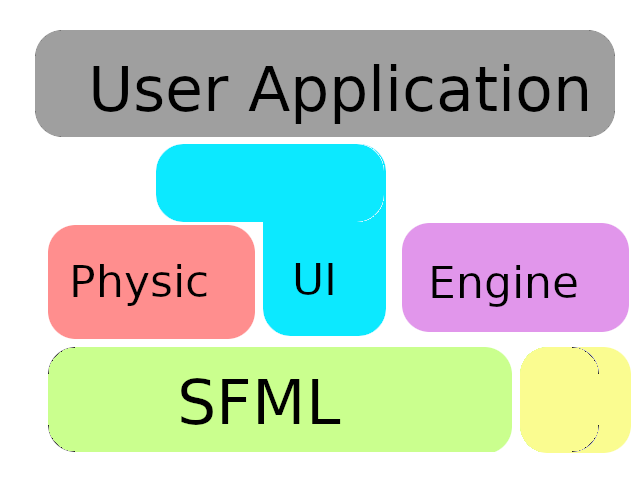
\includegraphics[width=0.8\linewidth]{model}




\end{document}
